Après avoir choisi les composants à partir du cahier des charges, nous avons sélectionné les GPIO importants pour envoyer des données à chaque composant.

Afin de schématiser tout cela, nous avons utilisé le logiciel Fritzing qui nous a permis de relier les composants virtuellement assez rapidement. Vous trouverez le schéma Fritzing ci-dessous.

\bigbreak
\begin{figure}[h]
    \centering
    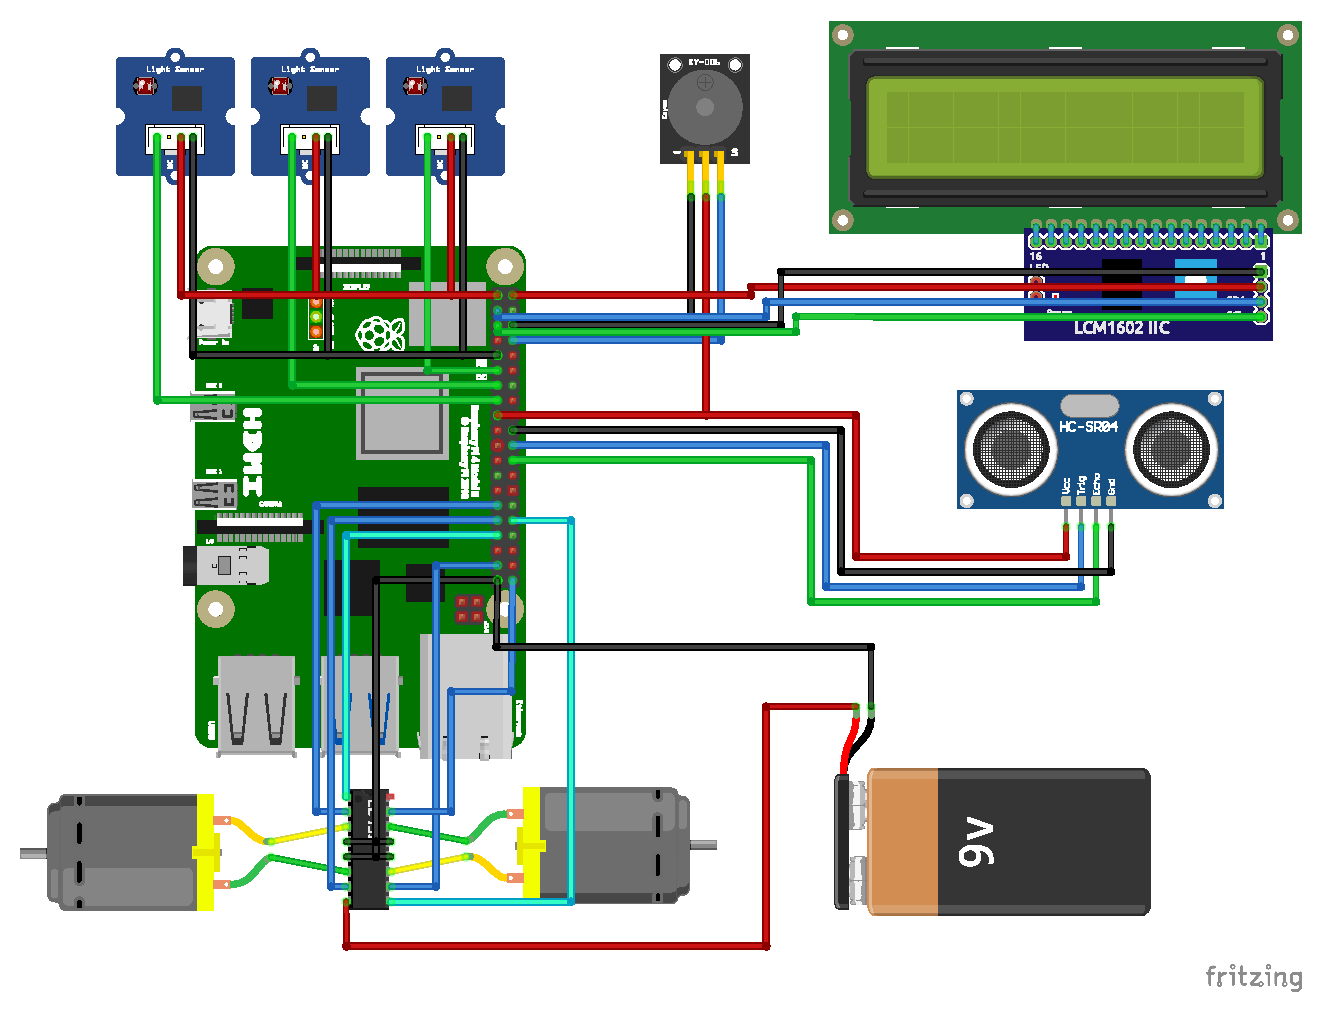
\includegraphics[width=1\textwidth]{fritzing/schema_composants.pdf}
    \caption{Schéma avec les composants Fritzing}
    \label{fig:Schéma des composants Fritzing}
\end{figure}

\begin{figure}[h]
    \centering
    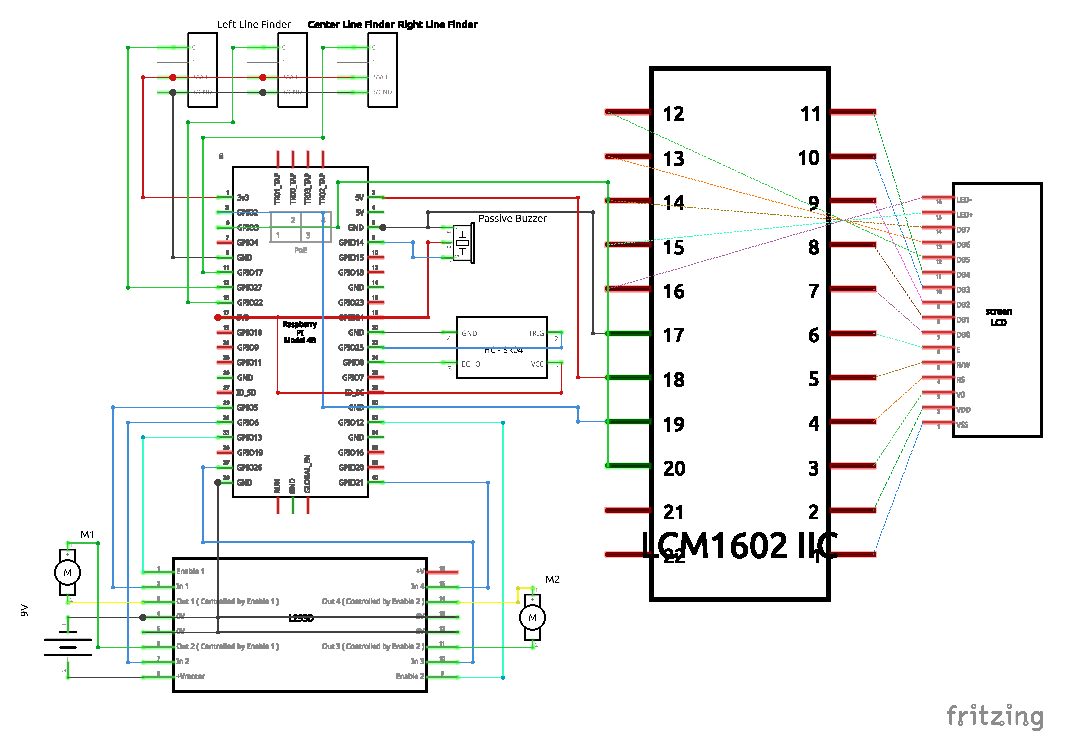
\includegraphics[width=1\textwidth]{fritzing/schema_electrique.pdf}
    \caption{Schéma électronique Fritzing}
    \label{fig:Schéma électronique Fritzing}
\end{figure}

\clearpage